\documentclass[10pt,a4paper]{article}
% %%%%%%%%%%%%%%%%%%%%%%%%%%%%%%%%%%%%%%%%%%%%%%%%%%%%%%%%%
% number of words:
% $ pdftotext file.pdf - | egrep -E '\w\w\w+' | iconv -f ISO-8859-15 -t UTF-8 | wc
% %%%%%%%%%%%%%%%%% metadata %%%%%%%%%%%%%%%%%%%%%%%%%%%%%%

\title{\bfseries{ \bf Minimalizácia štýlových predpisov v jazyku CSS}}
\author{Ján Antala}
\date{\today}

% %%%%%%%%%%%%%%%%%% definitions %%%%%%%%%%%%%%%%%%%%%%%%%%%%%

\usepackage{a4wide}
\usepackage{ucs}
\usepackage[utf8x]{inputenc} \usepackage[slovak]{babel}
\usepackage[slovak]{babel}

\usepackage{ae}
\usepackage{placeins}
\usepackage[pdftex]{graphicx}
\usepackage{fancyvrb}
\usepackage{listings}
\usepackage{url}
\usepackage{multirow}
\usepackage{lscape}
\usepackage{longtable}
\usepackage{setspace}

\usepackage{amsmath}
\usepackage{listings}
\usepackage{color}
\usepackage{textcomp}
\usepackage{url}

\usepackage{pslatex}
\usepackage{charter} 

\usepackage{lmodern}
\usepackage[svgnames]{xcolor}
\usepackage{listings}
% \usepackage{subfig}
\usepackage{graphicx}
\usepackage{caption}
\usepackage{subcaption}
\usepackage{verbatim}
\usepackage{float}
\usepackage[stable]{footmisc}
\captionsetup{justification=centering}

\selectlanguage{slovak}
\usepackage[numbers]{natbib}
\usepackage[titletoc]{appendix}

\addto\captionsslovak{\renewcommand{\appendixname}{Príloha}}
\rmfamily

% %%%%%%%%%%%%%%%%%%%%% MACROS %%%%%%%%%%%%%%%%%%%%%%%%%%%%%%


\newenvironment{fancy_enumerate}{
\begin{enumerate}
  \setlength{\itemsep}{1pt}
  \setlength{\parskip}{0pt}
  \setlength{\parsep}{0pt}}{\end{enumerate}
}
           
\newenvironment{fancy_itemize}{
\begin{itemize}
  \setlength{\itemsep}{1pt}
  \setlength{\parskip}{0pt}
  \setlength{\parsep}{0pt}}{\end{itemize}
}

 
\newsavebox{\selvestebox}
\newenvironment{fancybox}
{
  \newcommand\colboxcolor{F0F0F0}%F8E0E0
    \begin{lrbox}{\selvestebox}%
      \begin{minipage}{\dimexpr\columnwidth-2\fboxsep\relax}
        \vspace{0,15cm} 
          \hspace{0,1cm}
            \small \texttt \\
}
{ 
            \texttt \normalsize
          \hspace{0,1cm} 
        \vspace{0,3cm}
      \end{minipage}
    \end{lrbox}%
  \begin{center}
    \colorbox[HTML]{\colboxcolor}{\usebox{\selvestebox}}
  \end{center}}

\newcommand{\tab}{\hspace*{2em}}

\newcommand{\listxml{\lstset{
	backgroundcolor=\color{lbcolor},
	tabsize=4,
	rulecolor=,
	basicstyle=\scriptsize,
	upquote=true,
	aboveskip={1\baselineskip},
	columns=fixed,
	showstringspaces=false,
	extendedchars=true,
	breaklines=true,
	prebreak=\raisebox{0ex}[0ex][0ex]{\ensuremath{\hookleftarrow}},
	frame=single,
	showtabs=false,
	showspaces=false,
	showstringspaces=false,
	identifierstyle=\ttfamily,
	keywordstyle=\bf,
	commentstyle=\texit,
	stringstyle=\textit,
	numbers=none,                   % where to put the line-numbers
	language=Xml
}}} 

\newcommand{\listjava{\lstset{
	backgroundcolor=\color{lbcolor},
	tabsize=4,
	rulecolor=,
	basicstyle=\scriptsize,
	upquote=true,
	aboveskip={1\baselineskip},
%	columns=fixed,
	showstringspaces=false,
	extendedchars=true,
	breaklines=true,
	prebreak=\raisebox{0ex}[0ex][0ex]{\ensuremath{\hookleftarrow}},
	frame=single,
	showtabs=false,
	showspaces=false,
	showstringspaces=false,
	identifierstyle=\ttfamily,
	keywordstyle=\bf,
	commentstyle=\texit,
	stringstyle=\textit,
	numbers=left,                   % where to put the line-numbers
	language=Java
}}}

\makeatletter
\renewcommand\paragraph{\@startsection{paragraph}{4}{\z@}%
  {-3.25ex\@plus -1ex \@minus -.2ex}%
  {1.5ex \@plus .2ex}%
  {\normalfont\normalsize\bfseries}}
\makeatother

\definecolor{lbcolor}{rgb}{0.9,0.9,0.9}
\oddsidemargin 0.5cm


\begin{document}


%%%%%%%%%%%%%%%%%%% CONTENT  %%%%%%%%%%%%%%%%%%%%%%%%%%%%


\newpage
% %%%%%%%%%%%%%%%%%% FRONT PAGE %%%%%%%%%%%%%%%%%%%%%%%%%%%%

\pagenumbering{roman}

\setlength{\parindent}{0cm}

\thispagestyle{empty}

\begin{center}
\begin{LARGE}
\textmd{
Slovenská technická univerzita v Bratislave\\
\vspace*{0.2cm}
Fakulta informatiky a informačných technológií  
}
\end{LARGE}

\vspace*{1.0cm}
\begin{Large}
\end{Large}

\end{center}

\vspace{5.5cm}

\begin{center}
{\Large \textmd{{Ján Antala}}}
\end{center}

\vspace{0.1cm}
\begin{huge}
\begin{center}
\textsc{Minimalizácia štýlových predpisov v jazyku CSS}
\end{center}
\end{huge}

\vspace{0.5cm}
\begin{center}
{\Large{\textmd{Evolučné algoritmy}}}\\
\end{center}

\vspace{5.5cm}

\begin{flushleft}

\large{máj 2013} \\
\large{\url{https://github.com/janantala/genetic-css-minify}}
\end{flushleft}


\newpage


\pagebreak

%%%%%%%%%%%%%%%%%%% TOC, (LOT, LOF)  %%%%%%%%%%%%%%%%%%%%%%%%%%%
\newpage
\setcounter{page}{1}
\thispagestyle{empty}

\setcounter{tocdepth}{3}
\tableofcontents
\listoffigures 

\thispagestyle{empty}
\thispagestyle{empty}


\newpage

\newpage

\onehalfspacing 
\setlength{\parindent}{1cm} 
\pagenumbering{arabic}
\setcounter{page}{1}

\newpage
\section{Zadanie}

Pomocou GA sa pokúste minimalizovať veľkosť štýlových predpisov v jazyku CSS, pričom vnútorná sémantika štýlového predpisu sa nezmení. 

Experimentujte s parametrami ako elitárstvo, pravdepodobnosť mutácie a kríženia, či veľkosť populácie. Dosiahnuté výsledky experimentov zanalyzujte a zdokumentujte.

\section{Úvod} % (fold)
\label{sec:_vod}
Minimalizovanie prenášaných dát cez internet je nesmierne dôležité. Ich nevyhnutnosť vzrastá najmä s nástupom mobilných zariadení a čoraz väčšom využívaní drahých mobilných dát. Priemerná veľkosť webovej stránky v roku 2012 bola 1.25 MB a pri súčasnom trende bude jej veľkosť 2 MB v roku 2014 \cite{size}. Jednou z možností minimalizovania prenosov je minifikácia zasielaného CSS súboru.

Kaskádové štýly (,,Cascading Style Sheets'' - CSS) je jednoduchý mechanizmus na vizuálne formátovanie webových dokumentov \cite{css}. Bol navrhnutý štandardizačnou organizáciou W3C. Zatiaľ boli vydané dve verzie špecifikácie: CSS1 a CSS2, v súčasnosti sa pracuje na verzii CSS3. Hlavným cieľom používanie CSS je oddelenie vzhľadu dokumentu od jeho štruktúry a obsahu.

Kaskádový štýl tvorí súbor pravidiel, ktorý sa skladá zo selektorov (napr. p, h2\ldots) a deklarácii (napr. color, padding, margin, font\ldots):

\begin{verbatim}
p { 
    color: black; 
    padding: 5px;
    margin-bottom: 5px;
    font-size: 14px;
}

h2 {
    color: black; 
    padding: 5px;
    margin-bottom: 10px;
    font-size: 22px;
}
\end{verbatim}

Cieľom minifikácie je zmenšiť veľkosť predpisu nielen odstránením bielych znakov, ale aj spojením duplicitných deklarácií pod jeden selektor. Výsledok minifikácie bude tvoriť nasledujúci stav:

\begin{verbatim}
p, h2 {
    color: black; 
    padding: 5px;
}

p {
    margin-bottom: 5px;
    font-size: 14px;
}

h2 {
    margin-bottom: 10px;
    font-size: 22px;
}
\end{verbatim}

V tomto jednoduchom príklade sme minifikáciou ušetrili veľkosť 27 znakov. Pri komplexnejších kaskádových štýloch sa ušetrená veľkosť bude zväčšovať. Spájanie selektorov však nemusí byť vždy úplne efektívne. Príkladom je použitie príliš dlhých názvov, ktoré bude dlhšie ako samotné deklarácie, a následným vytvorením nového spojeného selektora.

Problém je známy ako ,,Minimum Biclique Covering'' (minimálny bipartitný graf), ktorého riešenie je NP zložité \cite{orlin, min}. Na minifikáciu CSS súborov je použitý genetický algoritmus. Spôsob realizácie algoritmu je popísaný v nasledujúcej kapitole.

% section _vod (end)

\section{Algoritmus} % (fold)
\label{sec:algoritmus}

Algoritmus je naprogramovaný v jazyku JavaScript pre systém node.js. Na spracovanie CSS súburu do podoby objektov je použitá npm knižnica css\footnote{https://npmjs.org/package/css}.

\subsection{Fitness} % (fold)
\label{sub:fitness}

Fitness funkcia aktuálneho kaskádového štýlu sa vypočíta ako rozdiel veľkosti (počtu znakov) pôvodného CSS súboru a veľkosti aktualného štýlu. Čím viac sa nám podarilo kaskádový štýl minifikovať, tým bude mať väčšiu fitness.

\begin{verbatim}
fitness = pôvodná veľkosť CSS - aktuálna veľkosť CSS
\end{verbatim}

% subsection fitness (end)

\subsection{Selekcia} % (fold)
\label{sub:selekcia}

Na selekciu jedincov z populácie je možné vybrať z nasledujúcich algoritmov: turnaj alebo ruleta. Výber je možné realizovať v úvodných nastaveniach programu.

\subsubsection{Turnaj} % (fold)
\label{ssub:turnaj}

Selekcia turnajom je implementovaná pre veľkosť turnaja dva. Prebieha tak, že sa z populácie náhodne zvolia dvaja jedinci a z nich sa na základe fitness vyberie ten lepší.

% subsubsection turnaj (end)

\subsubsection{Ruleta} % (fold)
\label{ssub:ruleta}

Selekcia ruletou prebieha tak, že každému jedincovi prislúcha taká pomerná časť z celkového súčtu fitness všetkých jedincov, akú má fitness on sám. Čím má jedinec väčšiu fitness oproti ostatným v populácii, tým je jeho šanca na výber väčšia.

% subsubsection ruleta (end)

% subsection selekcia (end)

\subsection{Kríženie} % (fold)
\label{sub:kr_enie}

V algoritme je kríženie celkom komplexná záležitosť. Keďže nový jedinec musí obsahovať všetky pravidlá, tak je potrebné ho opraviť. Kríženie medzi dvoma jedincami prebieha tak, že sa zoberie polovica dĺžky prvého jedinca a pridá sa k nemu druhá polovica z druhého jedinca. Aby nechýbali niektoré pravidlá, tak sa k novému jedincovi pridá ešte druhá polovica z prvého jedinca a následne sa zlúčia všetky duplicitné selektory. Podobne to prebieha aj s druhým jedincom.

Samotnú pravdepodobnosť kríženia jedincov je možné nastaviť v nastaveniach algoritmu, pokiaľ kríženie neprebehne, tak sa vrátia pôvodní jedinci.

% subsection kr_enie (end)

\subsection{Mutácia} % (fold)
\label{sub:mut_cia}

V programe sú použité dva spôsoby mutácie: mutácia rozdelením selektorov a mutácia spájaním. Zakaždým sa náhodné zvolí typ mutácie a pravidlo kaskádového štýlu, pre ktoré sa mutácia uplatňuje. Pravdepodobnosti mutácie je možné nastaviť.

\subsubsection{Mutácia delenia} % (fold)
\label{ssub:rozdelenie}

Mutácia rozdelením je aplikovaná na zložený selektor. V prípade náhodneho výberu jednoduchého selektoru sa nič nevykoná.

\begin{verbatim}
p, h2 {
    color: black; 
    padding: 5px;
}

\end{verbatim}

Po jej aplikovaní na kaskádový štýl sa vytvoria dva nové selektory s rovnakými deklaráciami. V prípade existencie rovnakého selektora sa ich deklaracie spoja a nevznikajú tak duplicity. Výsledok mutácie bude nasledujúci:

\begin{verbatim}
p { 
    color: black; 
    padding: 5px;
}

h2 {
    color: black; 
    padding: 5px;
}
\end{verbatim}

% subsubsection rozdelenie (end)

\subsubsection{Mutácia spájania} % (fold)
\label{ssub:sp_janie}

V prípade mutácie spájaním sa náhodne zvolia dva selektory z kaskádového štýlu a následne sa zisťuje, ktoré deklarácie sú rovnaké a je ich tak možné spojiť pod jeden zložený selektor. Mutácia spájaním je opakom mutácie rozdelením.

\begin{figure}[H]
	\centering
	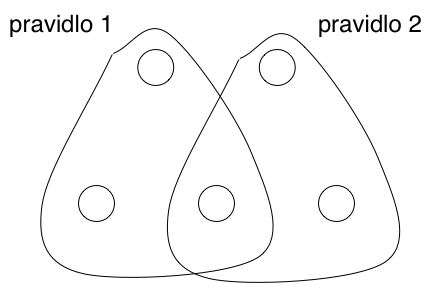
\includegraphics[width=0.5\textwidth]{rules.png}
	\caption[Možnosť spojenia dvoch pravidiel]{
		Možnosť spojenia dvoch pravidiel}
	\label{fig: rules}
\end{figure}

% subsubsection sp_janie (end)

% subsection mut_cia (end)

\subsection{Elitizmus} % (fold)
\label{sub:elitizmus}

Program umožňuje nastaviť množstvo najlepších jedincov z populácie, ktoré sa automaticky presunie do nasledujúcej generácie.

% subsection elitizmus (end)

\subsection{Koncový stav} % (fold)
\label{sub:koncov_stav}

Keďže sa jedná o špecifický druh úlohy tak koncový stav dopredu nepoznáme. Ukončenie algoritmu je tak možné dvoma spôsobmi: vyčerpaním maximálneho počtu generácii alebo prekročením limitu generácii, kedy sa fitness najlepšieho jedinca z populácie nezlepší. Oba parametre je možné nastaviť.

% subsection koncov_stav (end)

% section algoritmus (end)

% \newpage
\section{Experimenty} % (fold)
\label{sec:experimenty}

Experimenty boli vykonávané na reálnych CSS súboroch získaných na webovej stránke denníka SME. Menili sa rôzne parametre ako je veľkosť populácie, spôsob selekcie, elitizmus alebo pravdepodobnosť kríženia či mutácie a sledoval sa ich vplyv na vývoj fitness najlepšieho jedinca v populácii.

\subsection{Veľkosť populácie} % (fold)
\label{sub:ve_kos_popul_cie}

Experimenent veľkosti populácie prebiehal s nasledujúcimi parametrami, pričom sa skúmal vzťah medzi veľkosťou populácie a vývoja fitness.

\begin{verbatim}
var options = {
    populationLength: [5, 25, 50, 75, 100],
    maxGenerations: 10000,
    roundOut: 1000,
    mutateLine: 0.2,
    crossover: 0.2,
    elites: 2,
    selection: 'tournament'
};
\end{verbatim}

\begin{figure}[H]
	\centering
	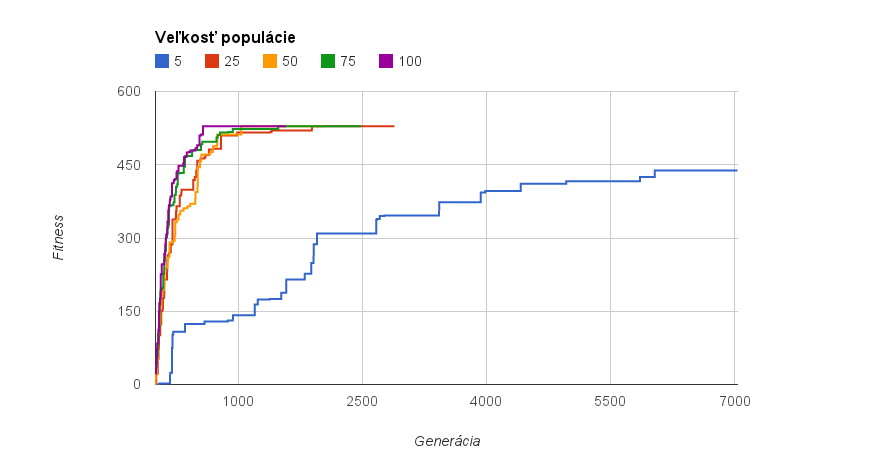
\includegraphics[width=1.0\textwidth]{population.png}
	\caption[Vývoj fitness v závislosti od veľkosti populácie]{
		Vývoj fitness v závislosti od veľkosti populácie}
	\label{fig: population}
\end{figure}

Ako najlepšia veľkosť populácie vzhľadom na rýchlosť zlepšovania fitness a dĺžku vykonávania programu vyznela populácia veľkosti 50. Pri malej populácii bola rýchlosť zvyšovania fitness pomalá a pri veľkej populácii sa jej rýchlosť už nezvyšovala, naopak zvyšovala sa dĺžka vykonávania programu.

% subsection ve_kos_popul_cie (end)

% \newpage
\subsection{Selekcia} % (fold)
\label{sub:selekcia}

Experimenent selekcie prebiehal s nasledujúcimi parametrami, pričom sa skúmal vzťah medzi druhom selekcie a vývoja fitness.

\begin{verbatim}
var options = {
    populationLength: 50,
    maxGenerations: 10000,
    roundOut: 1000,
    mutateLine: 0.2,
    crossover: 0.2,
    elites: 2,
    selection: ['tournament', 'roullete']
};
\end{verbatim}

\begin{figure}[H]
	\centering
	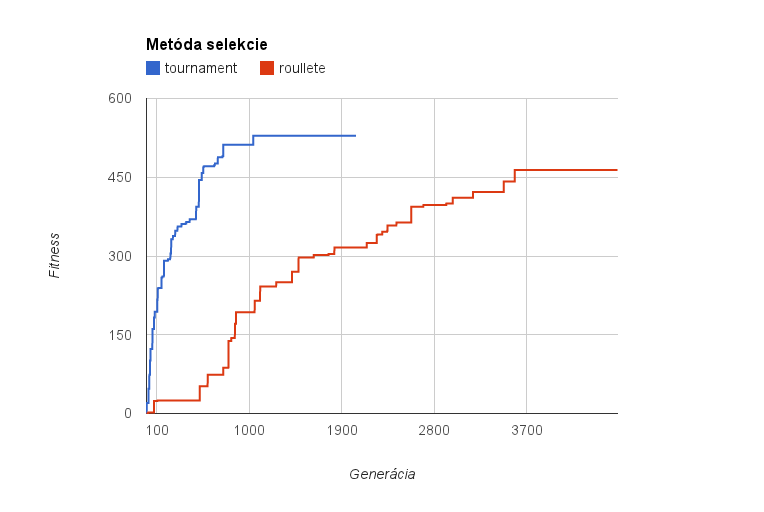
\includegraphics[width=1.0\textwidth]{selection.png}
	\caption[Vývoj fitness v závislosti od metódy selekcie]{
		Vývoj fitness v závislosti od metódy selekcie}
	\label{fig: selection}
\end{figure}

Lepší spôsob selekcie je selekcia turnajom. Selekcia pomocou rulety je časovo výrazne pomalšia a rýchlosť zlepšovania fitness najlepšieho jedinca v populácii taktiež dosahuje horšie výsledky ako selekcia turnajom.

% subsection selekcia (end)


% \newpage
\subsection{Elitizmus} % (fold)
\label{sub:elitizmus}

Experimenent elitizmu prebiehal s nasledujúcimi parametrami, pričom sa skúmal vzťah medzi počtom elít presunutých do nasledujúcej generácie a vývoja fitness.

\begin{verbatim}
var options = {
    populationLength: 50,
    maxGenerations: 10000,
    roundOut: 1000,
    mutateLine: 0.2,
    crossover: 0.2,
    elites: [0, 2, 10, 20, 30, 40]
    selection: tournament
};
\end{verbatim}

\begin{figure}[H]
	\centering
	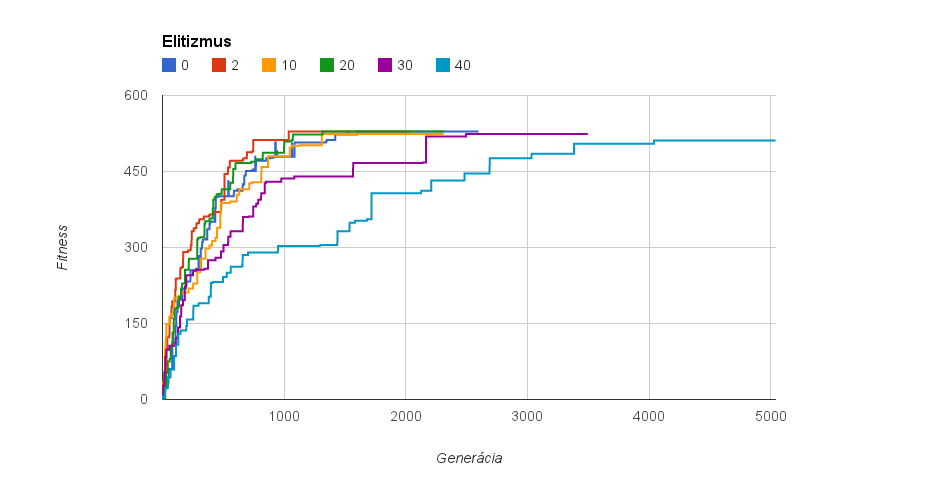
\includegraphics[width=1.0\textwidth]{elites.png}
	\caption[Vývoj fitness v závislosti od veľkosti elitizmu]{
		Vývoj fitness v závislosti od veľkosti elitizmu}
	\label{fig: selection}
\end{figure}

Z experimentu vyplýva, že v prípade malého presunutého počtu elít (v experimente sú to dvaja najlepší jedinci) do nasledujúcej generácie sa vývoj fitness zlepšuje najlepšie. Pokiaľ je elitizmus nulový, tak najlepšia fitness môže aj klesnúť. V prípade väčšieho elitizmu sa zlepšovanie fitness spomaluje.

% subsection elitizmus (end)

% \newpage
\subsection{Pravdepodobnosť kríženia} % (fold)
\label{sub:pravdepodobnos_kr_enia}

Experimenent kríženia prebiehal s nasledujúcimi parametrami, pričom sa skúmal vzťah medzi pravdepodobnosťou kríženia a vývoja fitness.

\begin{verbatim}
var options = {
    populationLength: 50,
    maxGenerations: 10000,
    roundOut: 1000,
    mutateLine: 0.2,
    crossover: [0, 0.2, 0.5, 0.75, 1]
    elites: 2
    selection: tournament
};
\end{verbatim}

\begin{figure}[H]
	\centering
	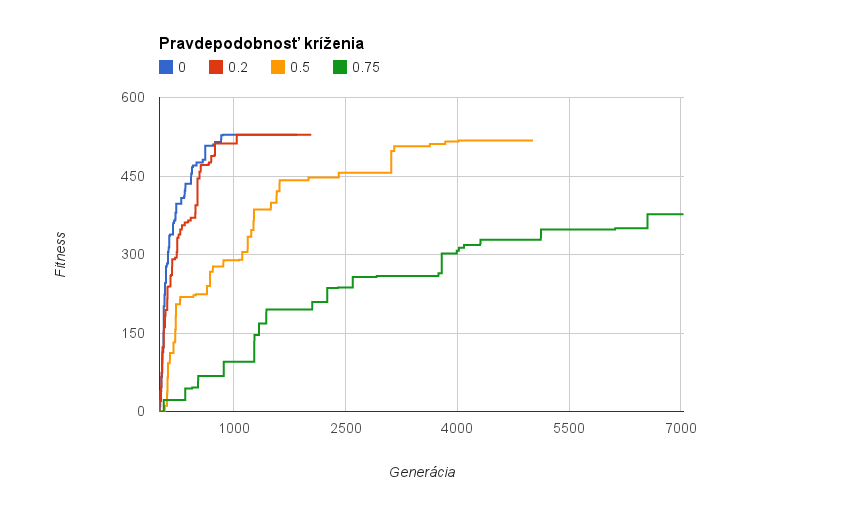
\includegraphics[width=1.0\textwidth]{crossover.png}
	\caption[Vývoj fitness v závislosti od pravdepodobnosti kríženia jedincov]{
		Vývoj fitness v závislosti od pravdepodobnosti kríženia jedincov}
	\label{fig: selection}
\end{figure}

Experimentom sa overil predpoklad, že pokiaľ je v algoritme zahrnuté kríženie, tak rýchlosť zvyšovania fitness sa zmenšuje. Je to spôsobené najmä tým, že po krížení jedincov často vznikne nový s väčšou veľkosťou ako bol pôvodný, pretože je potrebné zachovať všetky pravidlá selektorov a nového jedinca opravovať. Navyše so zvyšovaním pravdepodobnosti kríženia sa zvyšuje a dĺžka vykonávania programu.

% subsection pravdepodobnos_kr_enia (end)

% \newpage
\subsection{Pravdepodobnosť mutácie} % (fold)
\label{sub:pravdepodobnos_mut_cie}

Experimenent mutácie prebiehal s nasledujúcimi parametrami, pričom sa skúmal vzťah medzi pravdepodobnosťou mutácie a vývoja fitness. Mutoval každý zvolený jedinec a menil sa spôsob mutácie medzi rozdelovaním a spájaním selektorov pomocou parametra mutateLine. Ten označuje interval medzi rozdelovaním a spájaním, teda od 0 po mutateLine je pravdepodobnosť rozdelenia, od mutateLine po 1 je pravdepodobnosť spojenia.

\begin{verbatim}
var options = {
    populationLength: 50,
    maxGenerations: 10000,
    roundOut: 1000,
    mutateLine: [0, 0.2, 0.4, 0.6, 0.8, 1]
    crossover: 0
    elites: 2
    selection: tournament
};
\end{verbatim}

\begin{figure}[H]
	\centering
	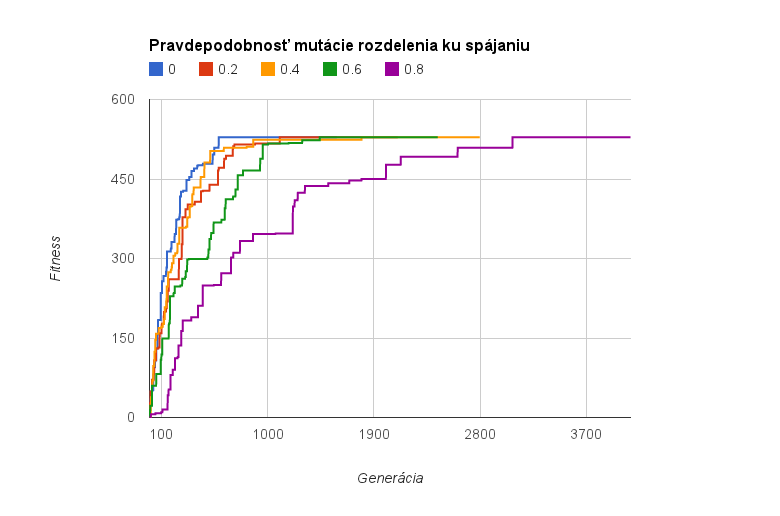
\includegraphics[width=1.0\textwidth]{mutation.png}
	\caption[Vývoj fitness v závislosti od pravdepodobnosti mutácie jedincov]{
		Vývoj fitness v závislosti od pravdepodobnosti mutácie jedincov}
	\label{fig: selection}
\end{figure}

Výsledkom experimentu je, že fitness najlepšie stúpa pri menšej pravdepodobnosti delenia a väčšej pravdepodobnosti spájania, aj keď presná hodnota dosť závisí od pôvodného CSS súboru.
% subsection pravdepodobnos_mut_cie (end)

% section experimenty (end)

% \newpage
\section{Obmedzenia programu} % (fold)
\label{sec:obmedzenia_programu}

Algoritmus v súčasnosti nepodporuje CSS3 selektory, ktoré vytvárajú vlastný priestor pôsobnosti, ale pracuje len z globálnymi selektormi. Medzi nepodporované patria napríklad @media alebo @keyframes a tak sú z pôvodného súboru ignorované.

Príklad nepodporovaných CSS pravidiel je nasledujúci, do algoritmu bude zahrnutý len prvý selektor ,,span''.

\begin{verbatim}
span { color: white; }

@media only screen 
and (min-device-width : 768px) 
and (max-device-width : 1024px) 
and (orientation : portrait) {
    span { color: red; }
}
\end{verbatim}

% section obmedzenia_programu (end)

\newpage
\section{Možné vylepšenia} % (fold)
\label{sec:mo_n_vylep_enia}

Okram dopracovania kompletnej podpory CSS3 selektorov existujú aj ďalšie vylepšenia programu. Medzi najdôležitejšie patrí zjednotenie duplicitných zápisov deklarácii zapísaných rôznymi spôsobmi. Príkladom je použitie farby:

\begin{verbatim}
p, div, span {	
    color: white; 
    color: #FFFFFF;
    color: rgb(255,255,255);
}
\end{verbatim}

Nastavenie farby by bolo možné aj jednoduchším zápisom:

\begin{verbatim}
p, div, span { color: white; }
\end{verbatim}

Farba však nie je jediným problémom. Ďalšími sú deklarácie ako ,,margin'', ,,padding'' či ,,border'', ktoré umožňujú vytvárať štýly pre každú stranu elementu a je ich možné zjednotiť do jednej. Problém reprezentuje nasledujúci príklad:

\begin{verbatim}
div {	
    margin-top: 10px;
    margin-bottom: 10px;
    margin-left: 10px;
    margin-right: 10px;
}
\end{verbatim}

Takýto zápis je možné zjednušiť pomocou jedného riadku:

\begin{verbatim}
div { margin: 10px; }
\end{verbatim}

Dlhodobejším cieľom je zapracovanie projektu ako vlastnej úlohy do nástroja Grunt\footnote{\url{http://gruntjs.com/}}, ktorý je v súčasnosti veľmi populárnym pri vývoji webového front-endu. Úloha by automaticky minifikovala vytvorený CSS súbor.
% section mo_n_vylep_enia (end)

\newpage
\section{Záver} % (fold)
\label{sec:z_ver}

Minifikácia CSS súborov bola úspešne testovaná na reálne nasadených projektoch. Použitím minifikátora sa podarilo zmenšiť ich celkovú veľkosť asi o 25\%. Z experimov sa zistili nasledujúce vlastnosti:

\begin{itemize}
\item najvhodnejšia veľkosť populácie je 50 jedincov
\item selekcia pomocou metódy turnaj
\item do nasledujúcej generácie je vhodné preniesť malý počet najlepších jedincov
\item kríženie nepoužívať, prípadne použiť len s malou pravdepodobnosťou
\item použiť mutáciu spájania selektorov s väčšou pravdepodobnosťou ako mutáciu rozdelovania
\end{itemize}

V súčasnosti sa však čoraz viac začínajú používať CSS3 selektory, ktoré nie sú v súčasnej verzii podporované. Preto je potrebné ich do plnej verzie zapracovať.

% section z_ver (end)


%%%%%%%%%%%%%%%%%%% BIB  %%%%%%%%%%%%%%%%%%%%%%%%%%%%  



\bibliographystyle{csplainnat}
\bibliography{bib.bib}

\end{document}
